    \begin{multicols}{2}
%%%%%%%%%%%%%%%%%%%%%%%%%%%%%%%%%%%%%%%%%%%%%%%%%%%%%%%%
%%%%%%%%%%%%%%%%% START 1_ARTICLE.tex %%%%%%%%%%%%%%%%%%
%%%%%%%%%%%%%%%%%%%%%%%%%%%%%%%%%%%%%%%%%%%%%%%%%%%%%%%%

%\chapter{Introduction}
\lettrine[lines=2]{\bfseries\color{black}D}{ual diagnosis} is the term used to describe the co-presence of a mental disorder and a substance use disorder in a single individual. It is a rather common occurrence, although actual numbers are uncertain and disputed. In the Danish context, it is often estimated that approximately 50\% of people in substance use treatment also have a mental disorder and approximately 30\% of people with a mental disorder will, at some point, have a substance use disorder (Flensborg-Madsen et al., 2009; Frederiksen, 2009; Toftdahl, Nordentoft, \& Hjorthoj, 2016). In other European countries the numbers seem to be a bit lower, in the US somewhat higher (Carrà, Bartoli, Brambilla, Crocamo, \& Clerici, 2015).
\par
Treatment for dual diagnosis in Denmark is divided between a medically based psychiatric treatment system and a socially oriented substance use treatment system, meaning that, in order to deliver the most effective treatment to people with dual diagnosis, the two systems need to cooperate.%
    \pagenote{In this article I write about ‘psychiatry’ and ‘substance use treatment’ as if they were coherent institutional units with common practices and values. That is of course an analytical simplification (some might even say an analytical violation). Psychiatry comprises many different things, substance use treatment even more. My reason for doing this, however, is that I want to focus my attention on the interface between psychiatry and substance use treatment. I want to develop an understanding of the complexity of that interface, not of the complexity of the two institutions trying to cooperate. Exploration of the complexity of psychiatry and substance use treatment respectively is the province of other articles.}
This has been emphasized in political statements (Sundheds- og Sundheds- og Ældreministeren, 2016) and bureaucratic guidelines, and a number of projects have been initiated to try out different models for cooperation, yet, on a larger, societal scale we have not solved the puzzle of how it can be made to work in practice. My focus in this article is to suggest some reasons why it is so difficult to introduce cooperation between psychiatry and addiction treatment despite the many projects explicitly directed towards doing so. In this analysis I draw upon the analytical framework of ‘organizational interfaces’ from organizational theory (Brown, 1983) to describe the cooperation between psychiatry and substance use treatment. However, I further develop Brown’s concept by explicating the hierarchical relations between the two organizations, thereby introducing power as an important dimension in understanding what is going on in the course of cooperation. Power, I should point out, is an issue that none of the projects have addressed explicitly.
\par
After this introduction, I briefly present why the constellation of mental and substance use disorders make up a special problem area, and then review the organization of the dual diagnosis field in Denmark more thoroughly. An introduction to the different cooperation projects on which I build my analysis in this article follows, including a discussion of my position as researcher and practitioner in the dual diagnosis field. In the ensuing analysis I describe current cooperation between psychiatry and substance use treatment before presenting some learning points that could guide future work in the dual diagnosis field. I conclude with a review of the analysis and my methodological approach. 

\chapter{The Problems of Dual Diagnosis}
Dual diagnosis patients are one of the groups that create difficulties for the treatment system and the way it is organized. This is the case not only in Denmark but throughout the Western world, where most existing research takes place (Carrà et al., 2015; Drake et al., 2016; Mueser, Noordsy, Drake, \& Fox, 2003). As an illustration, I begin by introducing Michelle, a woman with a dual diagnosis whom I met at a treatment facility (Johansen, 2009), before summarizing the different types of difficulties.
\par
Michelle had a very serious personality disorder and used a range of drugs, including heroin, cocaine and cannabis. She often had psychotic episodes after drug use or when she was stressed – frequent occurrences due to her drug habit. She lived in a small two-room flat with her boyfriend who, like Michelle, also had a personality disorder and used drugs; they financed their drug habit by dealing and Michelle’s having sex with men for money. Michelle had many – often negative – contacts with different treatment facilities. She was registered at a drug treatment facility where she received methadone for her heroin addiction, but because of her chaotic lifestyle she often missed her appointments and was reduced in dosage because of no-shows. This made her contact with drug treatment a largely negative experience, as most of it was about methadone doses. Furthermore, she had a preference for injecting her methadone when possible and it created conflicts when she could not take it home with her but had to take it at the treatment facility. Staff members strongly doubted whether all the conflict was due to her personality disorder. They had tried to refer her to the psychiatric treatment system but she was rejected as she could not be diagnosed properly due to her frequent drug intoxication, and because there was no treatment for patients with personality disorders if they were using drugs at the same time. She was told to return when she had been clear for some months. She was, however, often in contact with the psychiatric emergency room when she became psychotic. No long-term contact with psychiatry was established on the basis of these visits as Michelle was always eager to leave the facility as quickly as possible to return to her boyfriend and the drugs. Due to her lifestyle and the drug use Michelle’s physical health was also in poor condition. She had no contact with her general practitioner after she had been forbidden to visit the consultation for threatening the doctor in an attempt to have him prescribe benzodiazepines for her. Staff at the drug treatment facility tried on a number of occasions to establish cooperation with the psychiatric treatment system but this was always declined on the basis that, firstly, Michelle was not a patient of theirs and, secondly, that she was not properly diagnosed as her diagnosis had been made by the doctor at the drug treatment facility who specialized in general medicine, not by a psychiatrist.
\par
The difficulties with dual diagnosis lie at three different levels in the Danish context: that of the individual patient/client, of organization and of cooperation:
\par
\textit{Patient/client level}: Dual diagnosis patients have more serious symptoms and a poorer prognosis than those with only a mental or substance use disorder, as the two disorders apparently mutually reinforce each other, interacting in complex ways that impact both medical and social treatment (Helsedirektoratet, 2012; Johansen, 2009; Mueser et al., 2003).
\par
\textit{Organizational level}: The division of the treatment system between psychiatric and substance use treatment creates uncertainty about which system has treatment responsibility for a particular patient. The psychiatric treatment system has a history of rejecting or discharging people with co-occurring substance use problems and the substance use treatment system has traditionally not had the competencies to diagnose and treat mental health problems (Johansen, 2009; Merinder, 2007).
\par
\textit{Cooperation level}: The two systems have difficulties cooperating for several reasons: differences in treatment approach, professional culture / language and in legal terms; a lack of incentives supporting cooperation and thus often an absence of management support; and no common IT systems frequently combined with physical distance between the units (Johansen \& Børsting-Andersen, 2015; Regeringens Udvalg vedrørende Psykiatri, 2013; Rambøl \& Implement, 2017).
\par
The difficulties linked to the interactions of mental disorder and substance use disorder and its patients are not unique to the Danish context, and are thoroughly described in the literature (Drake et al., 2006; Mueser et al., 2003). The difficulties linked to different professional cultures are also well described (ibid.). There is considerable literature discussing cooperation problems between specialized, hospital-based psychiatry and more community-based interventions (Bengtsson, 2011; Folker et al., 2017; Johansen, Larsen, \& Nielsen, 2012; Ware, Tugenberg, Dickey, \& McHorney, 1999).%
    \pagenote{In much of this literature the focus has been on ‘continuity of care’ (Ware et al., 1999). However, when dealing with the dual diagnosis field the discussion seems to focus on how we can integrate psychiatry and substance use treatment, and integrated treatment seems to be the keyword (Mueser et al., 2003).}
However, Denmark has created a treatment system where we experience the full force of the difficulties. In the following section I look more closely at the organization of dual diagnosis treatment in Denmark.

\chapter{The Dual Diagnosis Field in Denmark}
From the time when psychiatry was established as a professional discipline at the beginning of the 18th century up until the 1960s, substance use disorders – primarily alcoholism and morphinism – were conventionally considered mental disorders that should be treated in psychiatry along with other disorders such as schizophrenia, bipolar disorder and depression (Kragh, 2015). But in the 1960s and 1970s Denmark removed substance use disorders –--especially drug use disorders--- from the field of psychiatry, making them the object of a growing field of social substance use treatment (Houborg, 2014; Winsløw, 1984). Alcohol use disorders were not removed in quite the same way; the psychiatric treatment system retained the task of treating acute alcohol intoxication, while more long-term therapy became the task of general practitioners and, later, treatment facilities located in the municipality or private agents.
\par
The division between medically based psychiatry and socially oriented substance use treatment that was established in those years is still maintained in Denmark. Psychiatry is part of the health care system and, as such, it is the responsibility of the Danish regions (of which there are five); the treatment system consists of emergency rooms, closed and open wards, and district mental health centers offering outpatient treatment. Outside of the hospitals we find privately practicing psychiatrists and psychologists. All these are defined as specialized treatment, while non-specialized psychiatric treatment is offered by general practitioners. Apart from psychologists, treatment is free, with access to the psychiatric treatment system being gained either by referral from a general practitioner or from the emergency units. Substance use treatment, on the other hand, is the responsibility of the municipalities (of which there are 98 in Denmark). Many municipalities have their own substance use treatment facility, while some buy services from other municipalities or private agents. Most treatment slots are for outpatients; in-patient treatment demands referral by the municipality. Substance use treatment in Denmark consists of both social interventions and – if appropriate for the substance use in question – medical intervention (for example, substitution treatment).
\par
There only exist a few specialized treatment facilities for dual diagnosis in Denmark – most of them located in the Capital Region – and the majority of people with dual diagnosis will receive psychiatric and substance use treatment separately (if they receive treatment at all). Yet the division of the treatment system contradicts a range of different recommendations for dual diagnosis, all of which advocate integrated treatment in which both the psychiatric and the substance use disorder are treated at the same time (see, for example, Helsedirektoratet, 2012; NICE, 2011, 2016). Another characteristic of the division is that it exists at all levels: from frontline staff, through organizational units, to the authorities, the law, ministries and so on. There is no place in the bureaucratic hierarchy where the two elements come together, no one who has joint responsibility for the dual diagnosis field, and therefore no one who can make a final decision on, for example, whose responsibility it is to provide proper treatment for a patient like Michelle.
\par
At the same time, there is considerable political and bureaucratic interest in the field, recently exemplified by a new guideline issued by the Danish Health Authorities in December 2016 that references the division between substance use treatments and psychiatry, and the concomitant need for cooperation (Sundhedsstyrelsen, 2017). Another example is a project that the Ministry of Innovation ran in 2017 identifying different ways that digitalization could support cooperation between substance use treatment and psychiatry (Rambøl \& Implement, 2017). In December 2017 the Ministry of Health announced that it was looking at models for another way of organizing the dual diagnosis field (Sundheds- og Ældreministeriet, 2017). In March 2018, the Danish Regions and some partners published their idea of what this could look like, suggesting that the psychiatric treatment system take over the responsibility of dual diagnosis treatment (Lægeforeningen, Dansk Psykiatrisk Selskab, Bedre Psykiatri, \& Danske Regioner, 2018).
\par
In Denmark, the situation is often described as one in which the dual diagnosis patient falls between two stools – that of substance use treatment and psychiatry; talking about the interstices between welfare service organizations is a case in point, as clearly illustrated by Michelle’s case. Political and bureaucratic levels have tried to deal with this in the Danish context by calling for cooperation – better cooperation and more of it (Regeringens Udvalg vedrørende Psykiatri, 2013) – meaning that many projects focusing on initiating and supporting cooperation have been carried out in recent years.
\par
If we look at the joint dual diagnosis field in terms of treatment initiatives and projects, it is possible to develop the typology presented below of different categories of treatment and cooperation within it.
    \begin{enumerate}
        \item Actual treatment units providing integrated treatment.
        \item The extension of one kind of current treatment to include aspects of the other mode: when substance use treatment also provides, for example, treatment for anxiety; or the community psychiatric center offers groups focusing on substance use. This often has an ad hoc character depending on locally experienced needs and/or the competencies of local staff.
        \item The employment of staff from one sector in the other sector: for example, when substance use treatment facilities hire psychiatrists or when nurses with expertise in substance use are hired in psychiatry.
        \item The establishment of formal and obligating cooperation. This mode can be further subdivided into the following levels (Socialstyrelsen \& Sundhedsstyrelsen, 2015):
            \begin{itemize}
                \item Exchange of information;
                \item Stable patterns of cooperation;
                \item Coordinator;
                \item Cross-sectional teams; 
                \item Organizational integration.
            \end{itemize}
    \end{enumerate}
The first two categories, as already mentioned, run counter to the official organization of the field in Denmark, and no publicly funded projects have been carried out focusing on these types of interventions. We do, however, find a few treatment units, both regional and local, providing integrated treatment (Category 1) or more informal adjustment of treatment methods (Category 2). The institutions found under Category 1 are exceptions in Denmark. Their establishment and continued existence is often linked either to visionary leaders promoting this kind of treatment, or a local institutional history wherein the profound need for a facility that could contain dual diagnosis patients, often with behavioral problems, was experienced. The different projects that have been carried out in the last couple of years (presented below) all fall into the third and fourth categories.
 
\chapter{Empirical Material}
My analysis draws on two different sources of empirical material. In my current position, I work as head of the Competence Centre for Dual Diagnosis (CCDD) in the Mental Health Services in the Capital Region in Denmark. The CCDD is a small department working with research and development within the dual diagnosis field. That means that I am both a researcher with a background in social anthropology and a practitioner in the dual diagnosis field, working with the organization of the field and competence development among staff, as well as research. That puts me in a unique position to gather knowledge and empirical examples, resulting in a deep understanding of the field and the challenges it contains (Watson, 2011; Ybema, Yanow, Wels, \& Kamsteeg, 2009). This means that I have a very privileged position in terms of conducting participant observation – the traditional data-generating method in anthropology. One of the challenges of participant observation is to find the proper balance between participating and observation (O'Reilly, 2005). This is no less of a challenge when one is a salaried and integral element of the observational field. Alvesson, who encourages the conduct of fieldwork in one’s own organization due to the intimate knowledge and easy access thus provided, writes of the concept of participant observation: 
    \blockquote[2009, p. 4]{The person [the fieldworker] is thus not an ethnographer in the sense of being a ‘professional stranger’ (Agar, 1986) or a researcher primarily oriented to studying the specific setting. Participant observation is thus not a good label in this case; ‘observing participant’ is better at capturing the meaning I have in mind…. Participation comes first and is only occasionally complemented with observation in a researched-focused sense.}
This description resonates with my own experience. Another challenge – also described in detail in textbooks on ethnographic methods (Emerson, Fretz, \& Shaw, 2011) – lies in keeping meticulous fieldnotes, a challenge which does not decrease when one is part of the discussion, workshop or meeting, with no time afterwards to write it up. Consequently, I have a profound sense of the field and ‘the game’ of dual diagnosis in the Danish context, but not piles of notes to sort and code when working with an article like this.
\par
I do not have a clinical background. Therefore, I am part of the field without actually treating patients or clients; I can talk to them without checking for symptoms or signs of treatment success or failure, interact with them without having to act (except in extreme situations like the threat of suicide). Furthermore, I am in a situation in which both patients / clients and staff are my informants, with both perspectives equally important and equally valid. This means that, while I am not best qualified to describe and comprehend, for example, the clinical effect of a specific medical or therapeutical intervention, the anthropological perspective provides insight into social relations, cultural meanings and structures of power, all of which have equal importance if we want to understand what goes on in the dual diagnosis field (Watson, 2011; Ybema et al., 2009). In this article, this knowledge allows me to produce a thorough description of the context of the different examples and projects mentioned.
\par
The other type of data used in this article is drawn from a range of cooperation projects that have been carried out within the dual diagnosis field in Denmark from 2008-2017.%
    \pagenote{Besides these projects focusing on dual diagnosis there exists a number of other projects focusing on creating connection between different welfare services for people with mental health problems (Folker et al., 2017).}
The six projects presented here all took place in the Capital Region of Denmark, although projects have also been carried out in the four other regions; many of them along the same lines as the projects described here. Most have produced evaluation reports that describe the interventions and provide an impression of their success; these constitute the main part of my empirical material (I should mention that I have contributed to several of them). Two of the projects have not yet been officially evaluated and my knowledge of those stems from my involvement qua my position as head of CCDD.
\par
I want to emphasize that this is not a study of what actually goes on in interactions as staff from the fields of psychiatry and substance use treatment try to cooperate. I am working with another kind of data here: the reports of, and dialogue with, the practitioners who have been working with the specific projects, with the purpose of discovering what we can learn about the dual diagnosis field by looking at how the cooperation is described. As such, I am inspired by the approach described by Shore and Wright in their book, Anthropology of Policy (1997), and the research questions they perceive within this frame:
    \blockquote[1997: 3]{How do policies ‘work’ as instruments of governance, and why do they sometimes fail to function as intended? What are the mobilizing metaphors and linguistic devices that cloak policy with the symbols and trappings of political legitimacy? ... How are normative claims used to present a particular way of defining a problem and its solution, as if these were the only ones possible, while enforcing closure or silence on other ways of thinking and talking?}
In the same way, I am interested in the focus on cooperation in the different publicly funded projects and the lack of focus on the uneven power structures between the cooperating partners. The projects are very briefly summarized below.
\par
\textit{The Social Nursing Project} (Projekt Socialsygepleje – det gode patientforløb). This was part of a larger project in which nurses specializing in substance use treatment were placed in hospitals – both somatic and psychiatric. Their task was to facilitate better treatment for patients who also had a substance use disorder. The project was well evaluated at the somatic hospitals and continued in those locations after the project period finished. In the psychiatric departments, however, the social nursing project was not successful. The social workers in the psychiatric departments perceived the nurses from the project as competitors, and their competence in substance use treatment was not recognized by the psychiatrists. Furthermore, the psychiatric nursing staff experienced competition with the social nurses in making alliances with the patients (Ludvigsen \& Brünés, 2013).
\par
\textit{The Integrated Approach Project} (Projekt Integreret Indsats). This was a cooperation project involving one psychiatric hospital and two local municipalities. The project worked with seriously mentally ill people who were also in contact with social psychiatry and substance use treatment. The working method of the project comprised cross-sectional treatment meetings every other week, during which common clients/patients were discussed and a joint approach decided upon. The project found that these meetings created an integrated approach to the clients/patients that facilitated both cooperation and a better treatment outcome for the patients (Deloitte.Social, 2016). However, the project managers also reported that it was important that the cooperation received ongoing attention and that the different institutional cultures were addressed directly and continuously if cooperation were to be successful (Johansen \& Børsting-Andersen, 2015).
\par
\textit{The Clinic for Substance Use and Non-Psychotic Mental Disorder} (Klinik for misbrug og ikke-psykotiske sindslidelser). This was another cooperation project involving a different psychiatric hospital and seven municipalities, which was directed at dual diagnosis patients with non-psychotic disorders. The clinic was established at the psychiatric hospital and treatment staff from the local substance use treatment facilities were to join the work at the clinic. The project was rather un-successful. The psychiatry-based clinic did not manage to incorporate the staff or treatment approaches from substance use regimens. On the contrary, several of the approaches applied in substance use treatment were rejected with the explanation that they were not evidence-based and not sufficiently well described to be included in a psychiatric treatment facility. The project managers from the psychiatric hospital themselves conducted a literature survey and decided on screening instruments and treatment principles identified through this work. The psychiatric staff did not see the need to include the staff from the substance use treatment facilities, and the latter could not see why they should participate. Instead of cooperation, the project created a situation of competition among the participants (Buch, Thygesen, \& Johansen, 2015).
\par
\textit{The Cross-Sectional Team at a Social Psychiatric Housing Facility} (Fællesteam på botilbud). This was yet another cooperation project between a psychiatric hospital and a municipality. Two psychiatric nurses, a psychiatric consultant and two staff members from the local substance use treatment facility formed a team to provide integrated treatment of dual diagnosis to people living at a social psychiatric housing facility. The team reported having been able to include most residents in the treatment despite earlier problems with retention. Cooperation with the local psychiatric hospital was successful and facilitated more planned admissions, although the team experienced major obstacles to accessing the IT systems of the psychiatric hospital and the municipality, making cross-sectional work difficult. Despite good results, the team was shut down after the project period. The experience gained through this project was used to create two new cooperation projects.
\par
\textit{The Coordination Plan} (Den Koordinerende Indsatsplan). In 2014, the government issued new guidelines on what is called the Coordination Plan. This suggests that people who are in contact with both the psychiatric treatment system and the substance use treatment system should have such a plan, to be developed at a meeting between representatives for both treatment systems and the patient/client. Here it should be agreed upon ‘who would do what and when’, so that the different treatment initiatives could be coordinated. The Coordination Plan has been implemented in several projects but without marked success. Staff members find it demanding of resources to initiate and are often in doubt whether it is actually necessary to have such planning meetings, while it has proven difficult to get consent from some patients / clients (Buch \& Petersen, 2017). It has also been clear that psychiatry and substance use treatment systems have very different incentives for involving themselves in the work of implementing such plans. Substance use treatment operatives hoped that the Coordination Plan could work as a shortcut into psychiatry, thus avoiding standard visitation procedures and also assuring clients treatment in psychiatry, whereas the psychiatric treatment system primarily had an interest in assuring that this did not happen, thus safeguarding their limited resources. \par
\textit{The Joint Screening Project} (Screeningsprojekt på Frederiksberg). The last project to be mentioned is one focusing on screening for mental disorders at a local substance use treatment center. This type of project has been carried out several times in several places, resulting in an article describing a project instigated in Århus (Frederiksen, 2009); the Frederiksberg project that I discuss here is a duplicate. Staff at the local substance use treatment center use standardized screening tools for mental disorder. If they identify someone with problems, they can refer the client for further assessment by a psychiatrist at the local psychiatric hospital. This psychiatrist also makes an evaluation of relevant treatment possibilities and will refer the client to the correct treatment facility (most often psychiatry or a general practitioner). The project is positively evaluated by the participants. Among other things, they mention that the formalized cooperation makes informal exchange possible and facilitates counselling when necessary.
\par
Though these six projects are very different in size and scope they indicate the political interest in the field, meanwhile documenting how cooperation is seen as the main solution to the challenges of the dual diagnosis field. The projects are summarized in \tref{tab:1} below:
    \end{multicols}
\FloatBarrier
\noindent
\begin{table}[htb]
\centering
\caption{Overview over Projects and Problems Identified}
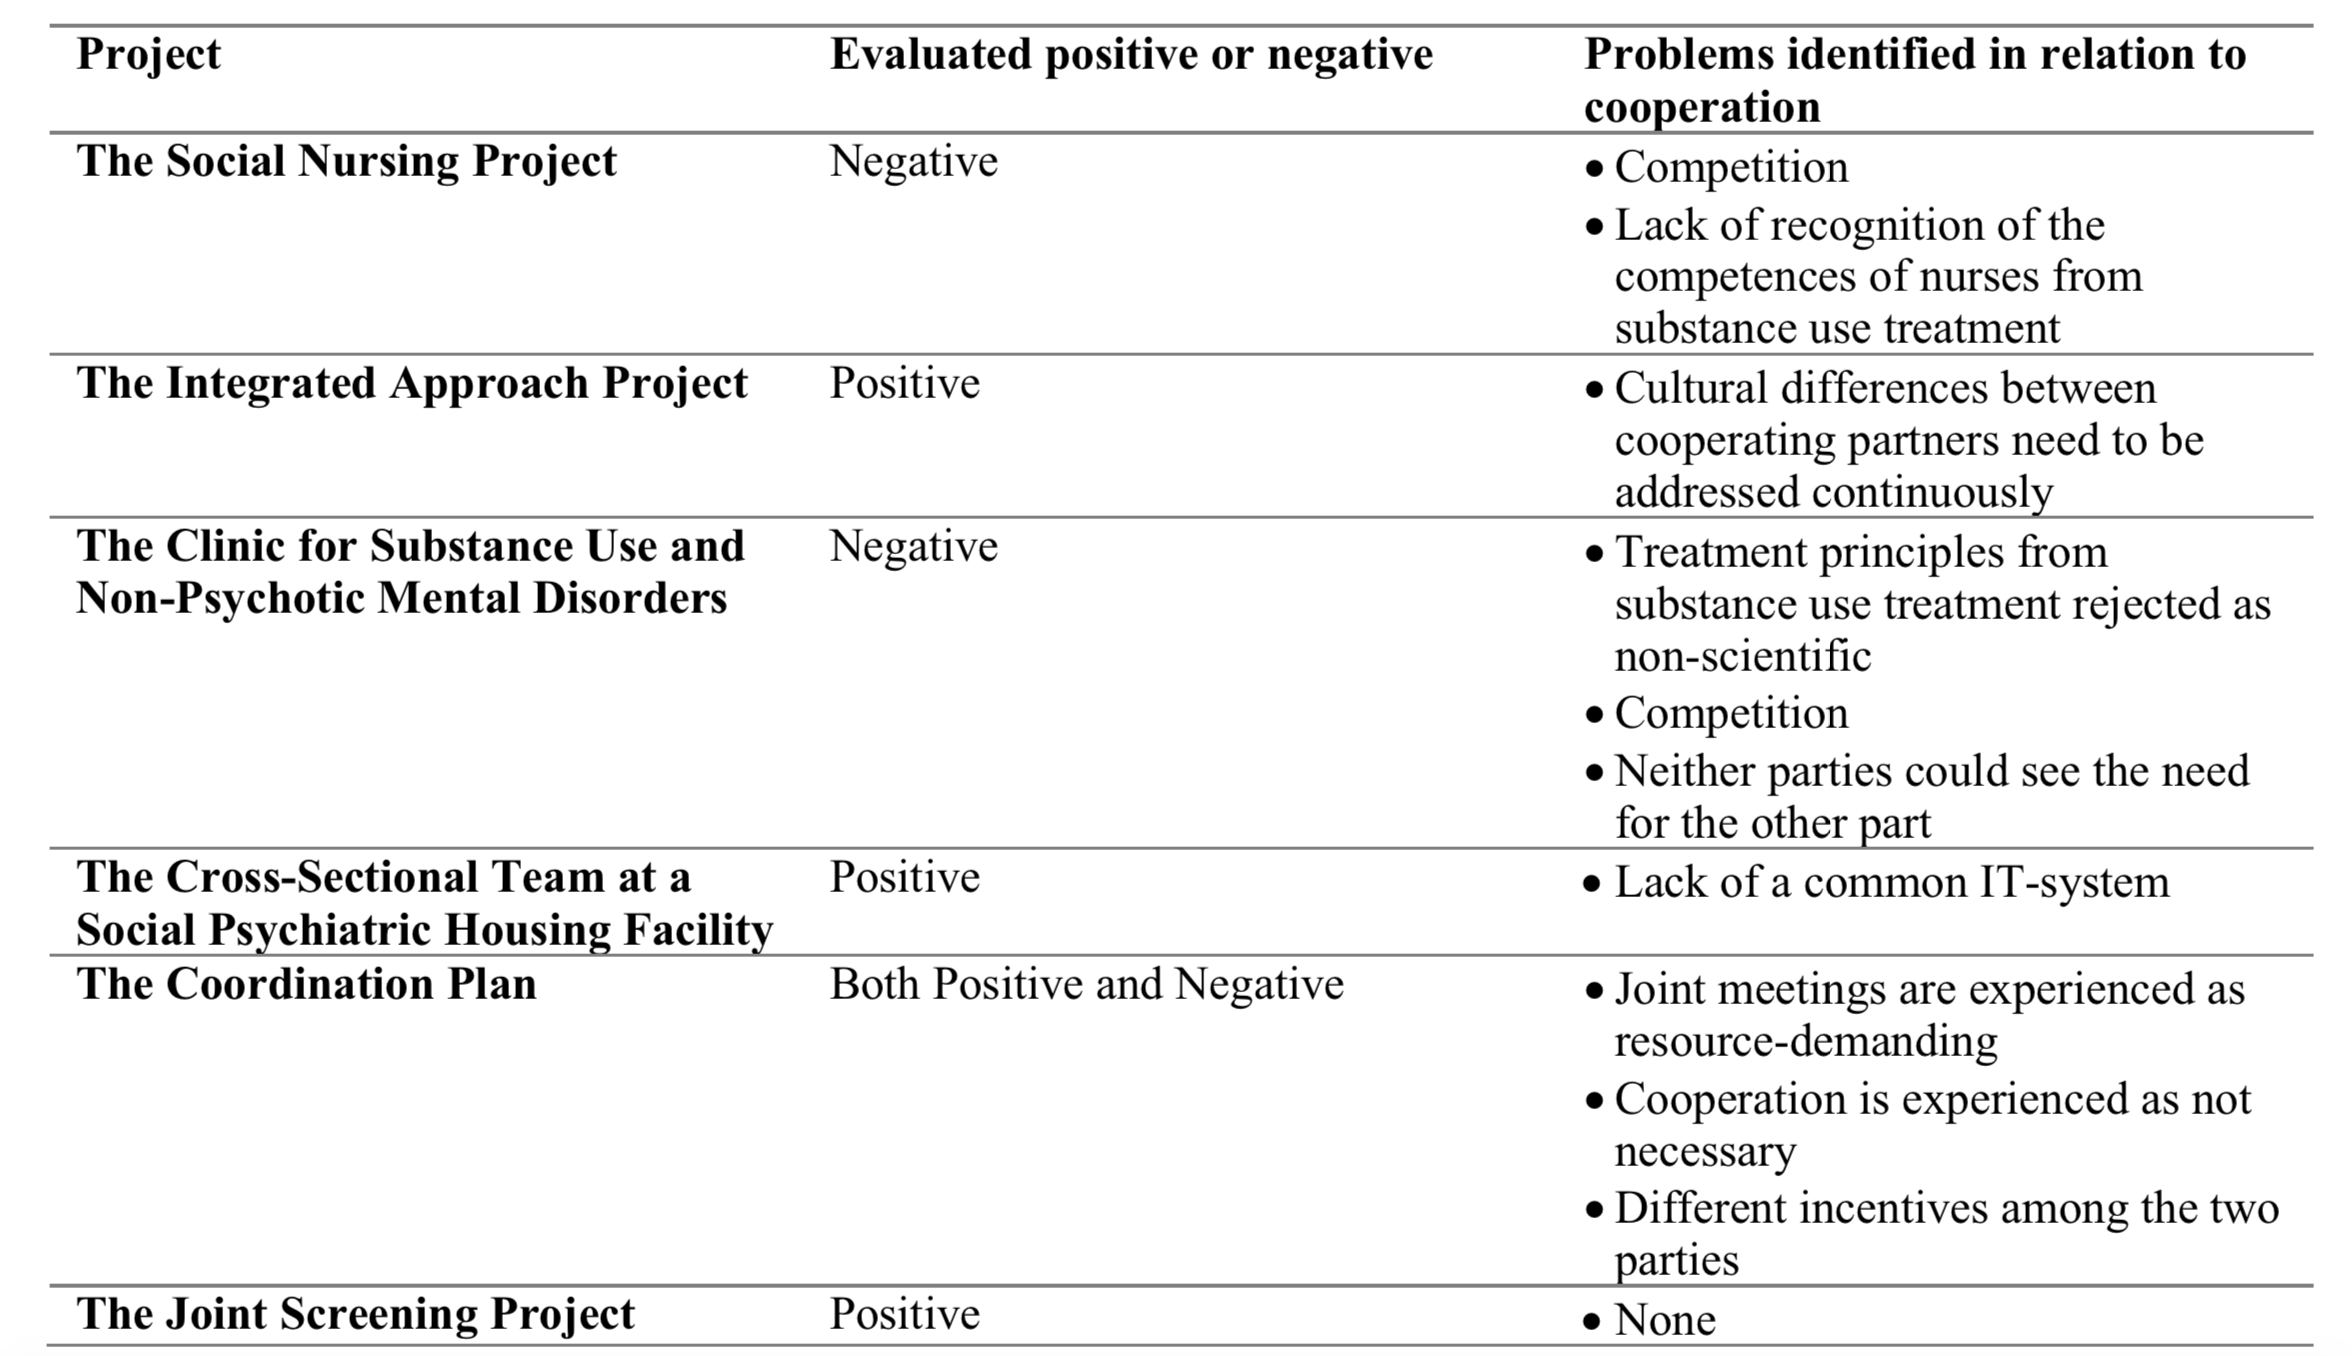
\includegraphics[width=0.9\linewidth]{paper6/p6_data/p6_tab1.png}
\label{tab:1}
\end{table}
\FloatBarrier
    \begin{multicols}{2}
\section{Cooperation Between Psychiatry and Substance Use Treatment --- Organizational Interfaces}
Organizational theorist David Brown has introduced the concept ‘organizational interfaces’ (Brown, 1983) that is central when analyzing cooperating organizations.%
    \pagenote{I have been introduced to David Brown’s work by Professor Janne Seemann from Ålborg University who has used his concepts in her own work with institutions, including psychiatric institutions, in the Danish welfare state (for example, Christensen, 2011; Seemann, 2008).}
Brown states that ‘[t]he definition of an interface depends on the shared goals and interdependencies that press parties to continue to act’ (1983: 22). He continues: 
    \blockquote[ibid.: 22--23]{Many organizational interfaces, for instance, are defined by shared tasks, for whose accomplishment the parties need each other. … Other interfaces are based on common social identifications. … Some interfaces are defined by acceptance of common authorities… still other interfaces are defined by physical space.}
In his approach there are four central elements that require analysis in order to comprehend organizational interfaces: 1) the interface itself; 2) the parties to the interface; 3) the party representatives; and 4) the larger context. If we apply Brown’s concepts to the Danish dual diagnosis field, we can produce the following model:
    \end{multicols}
\FloatBarrier
\noindent
\begin{figure}[htb]
\centering
\caption{The Danish Dual Diagnosis Field, version 1}
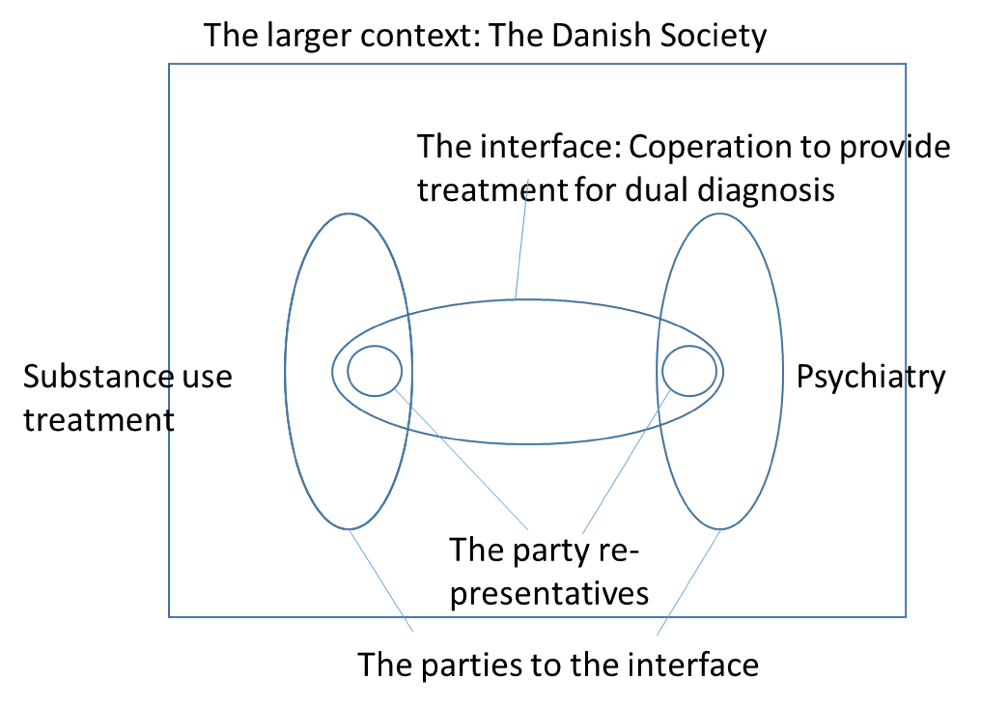
\includegraphics[width=0.9\linewidth]{paper6/p6_data/p6_model1.png}
\label{fig:model:1}
\end{figure}
\FloatBarrier
    \begin{multicols}{2}
If we look at the different projects through the lens of Brown’s organizational interfaces we can see that, to a large extent, they may be characterized by this concept. We can identify the interface between psychiatry and substance use treatment and we can identify the cooperating parties – psychiatry and substance use treatment. The party representatives in the different projects can be identified – whether they be social nurses, ordinary staff assigned to the project or project managers working with the projects – and likewise the context in which the cooperation takes place: the larger Danish society.
\par
In some of the projects, cooperation seemed rather successful and in line with Brown’s model. Staff from the two sectors seemed to agree that both parties are needed if proper treatment solutions are to be made. The Integrated Approach Project and The Cross-Sectional Team at a Social Psychiatric Housing Facility are examples of this.
\par
Yet some of the projects show quite another picture, one that makes Brown’s model seem too equable. Some of the projects clearly showed that the rationales for substance use treatment and psychiatry when entering into agreements of cooperation and joint project work are not necessarily the same. The rationale of those operating in substance use treatment seems to be a wish to gain access to psychiatric professionalism, diagnosis and treatment, as demonstrated by the project exploring the Coordination Plan. If one applies the definition of cooperation borrowed from Brown, then, from their perspective, there is a need for cooperation that is defined by a shared task – that of treating people with a dual diagnosis. The psychiatric field, on the other hand, does not seem interested in the professional perspective of substance use treatment, at least not to the same extent. In one project – The Clinic for Substance Use and Non-Psychotic Mental Disorder – psychiatry operatives dismissed the perspective of substance use treatment altogether when they characterized it as ‘not evidence-based’. In another project – The Social Nursing Project – the psychiatric staff did not seem to think that social nurses had anything to contribute. Rather, they seemed to be confident that they could manage dual diagnosis treatment quite well on their own. This points to asymmetrical power relations in the organizational interface wherein the psychiatric profession has the upper hand.
\par
There are probably several different explanations for this. One could be that psychiatry – as a specialized service with restricted access – represents a scarce and therefore more attractive resource than substance use treatment, which is a low threshold treatment mode open to everybody. Another obvious explanation is that psychiatry as a medical profession draws on the prestige of modern medicine, whereas substance use treatment in the Danish context is linked to the less prestigious field of social work: an issue throughout the otherwise successful Integrated Approach Project. The rejection of the approaches of substance use treatment with the argument that they were not evidence-based that we saw in the project with the Clinic for Substance Use and Non-Psychotic Mental Disorder is also an example of medicine being more prestigious than social work.
\par
Another characteristic of the Danish dual diagnosis field is, as mentioned in the introduction, that the division between psychiatry and substance use treatment exists on all levels – from frontline staff, through organizational units, to the authorities, the law and ministries – and none of these levels offers joint responsibility in the dual diagnosis field. That means that the context of the organizational interface does not really provide a frame for interaction, as the model presented above indicates.
\par
I would therefore suggest that the model for organizational interface, when it comes to the dual diagnosis field in Denmark, is more properly portrayed like this in some situations:
    \end{multicols}
    \FloatBarrier
    \noindent
    \begin{figure}[htb]
    \centering
    \caption{The Danish Dual Diagnosis Field, version 2}
    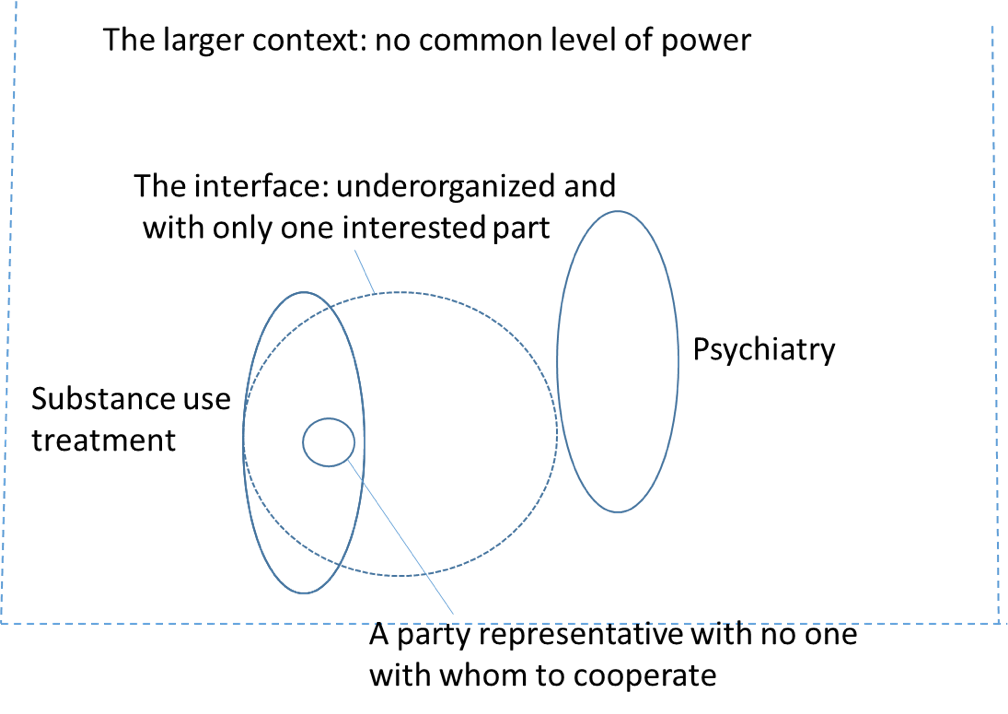
\includegraphics[width=0.9\linewidth]{paper6/p6_data/p6_model2.png}
    \label{fig:model:2}
    \end{figure}
    \FloatBarrier
    \begin{multicols}{2}
Most of the cooperation projects introduced above do not address this potentially conflictual cooperation situation, with the Integrated Approach Project being a partial exception as, half-way through the project, the project managers established a meeting forum for project participants where different institutional cultures, ethical questions and power relations were directly addressed (Johansen \& Børsting-Andersen, 2015). In the majority of the projects, the project designers and project managers seemed to think that the situation resembled that indicated in Model 1. For some of the projects this might have been true initially, but then, during the course of the project, the organizational interface developed into a situation more like that presented in Model 2. For other projects, the situation was probably more like Model 2 from the outset but without project designers and project managers addressing this issue in the project design and project work. This indicates that the organizational interface between substance use treatment and psychiatry is not static; rather, it can change over time. The actual manifestation of the interface will probably also depend on, for example, local organizational principles and histories of cooperation, among other elements.
\par
Model 1 and Model 2 can also be seen as the poles of a continuum, with most cooperation projects being placed somewhere between the two extremes, although tending to be placed closer to Model 2 if questions of differences in culture, language and power are not explicitly addressed (see also Johansen et al., 2012). 

\chapter{An Under-Organized Interface}
In Model 2 of the organizational interface, I introduce another of Brown’s analytical concepts – that of organizational interfaces as either underorganized or overorganized – neither of which is a positive outcome (1982: 28-30). An underorganized interface has the following characteristics:
    \blockquote[1982: 28]{There is little agreement about who has authority, and interface goals are undefined or conflicting. Formal regulatory mechanisms are not well-developed: Representative roles are fragmented, conflicted, of undefined, and procedures for handling issues are unclear or ineffectual. Informal mechanisms provide few clear constraints: Theories and values about the interface are not shared; representatives believe that chaos is imminent, some fighting or fleeing are appropriate; cultural differences based in the invading environment are more important than task differences.}
The dual diagnosis interface can best be described as underorganized (see also Christensen, 2011), and the underorganized interface creates a range of problems. In Brown’s words: 
    \blockquote[1982: 28]{Several problems are characterized within underorganized interfaces. Resources are typically in short supply; the interface lacks personnel, information, energy and time. Available energy is diffused by the lack of clear focus and the everpresent potential for leaving the system. Finally, differences easily lead to two forms of negative conflict permitted by loose organization: (1) withdrawal from differences and (2) escalation of conflict.}
Again, we find these characteristics in the different projects described above. Some of the agents – in my material primarily psychiatric staff – do seem reluctant to invest in the interface, seeming to prioritize using their resources within their own system. In two of the projects – The Clinic for Substance Use and Non-Psychotic Disorders and The Social Nursing Project – we saw a situation with a high level of conflict between the two parties.
\par
It is also tempting to understand the concept of underorganized in a slightly different way than Brown, however. Suggesting that a field is underorganized could also describe a situation in which there is room for a range of local initiatives and projects. The above lists of treatment initiatives and projects and models of cooperation could thus be seen as the result of the underorganization of the field: as formal regulations for the interface are lacking and as there is no formal structure to regulate the dual diagnosis field, local initiatives are created in an attempt to fill its interstices. On the one hand this could be seen as positive – there is room for local initiatives and models for cooperation. But I suggest that the underorganized character of the field, resulting in the large number and variety of local initiatives, add a further level of difficulty to the dual diagnosis field. Not only do we have those connected to patient/client organization and cooperation mentioned in the introduction to this article, the many different initiatives also create a field characterized by randomness and changeability.

\chapter{Learning Points}
Based on the included projects and the analysis of the interface it is possible to identify some elements in the projects that could assist in the direction of policy-making.
\par
In The Integrated Approach Project, as already mentioned, the project managers became aware that they needed to address the cultural differences between the participating parties (in this case, psychiatry, substance use treatment and social psychiatry). In their experience, staff members from the different sectors wanted to cooperate but, when facing difficult cases or situations, they often withdrew to more traditional and therefore safer positions – focusing on the core tasks of their own institution and not on cross-sectional cooperation. In their experience, the cultural differences need continuous attention if this withdrawal from cooperation is to be avoided (Johansen \& Børsting-Andersen, 2015). Examples of activities addressing this problem are cross-sectional competence development, cross-sectional supervision and the involvement of relevant leaders in supporting the cross-sectional work (see also Johansen \& Wiuff, 2014).
\par
Another positive example from the projects listed above is The Cross-Sectional Team at a Social Psychiatric Housing Facility. They successfully established a team that worked well together, where the different perspectives of the involved staff members were fully integrated, thereby providing evidence that such a setup is possible, at least under certain conditions. It is worth noting that the staff members working in this project were very experienced in their respective professions. Moreover, the Cross-Sectional Team worked as a relatively small, autonomous unit away from the institution of origin and well-established power relations. One could claim that, in consequence, it did not challenge institutional structures or power hierarchies. In other words, it was not dangerous and its members could be left to work together rather undisturbed. As also pointed out, the project was not continued after the project period ran out and the experiences were not used to change the treatment systems.
\par
In the course of The Joint Screening Project successful cooperation was also established. It is a characteristic of that project that it does not challenge structural borders or the competencies of psychiatry. On the contrary, it is built on a recognition of psychiatrists’ possessing an exclusive knowledge of mental disorders that substance use treatment can only access through a psychiatrist. The services provided by the psychiatrists hired in the project are very specific and delimited.
\par
To summarize: if we do not want to change the organization of the dual diagnosis field but are only aiming for more successful cooperation, the above analyzed projects seem to point to three different models of cooperation:
    \begin{itemize}
        \item Autonomous units consisting of experienced professionals working out their own approach;
        \item Recognition of psychiatry as the dominant element and a concomitant adaptation of cooperation patterns to accommodate this;
        \item Continuing insistence that cooperation is possible – meanwhile providing time, resources and space for the participants to develop a fully cooperative culture.
    \end{itemize}
These are pragmatic suggestions and their ability to change the basic structures of the dual diagnosis field are limited. 
\par
The analysis presented above indicates that one of the reasons why it seems difficult for psychiatry and substance use treatment to cooperate is that the two institutions do not enter into cooperation on equal terms and do not seem to agree on its necessity.
\par
While I was writing the first draft of this article in January 2018, the Ministry of Health issued a policy paper suggesting that the regions should take over responsibility from the municipalities for substance use treatment for people with dual diagnosis. The purpose of this would be to secure a better quality of treatment for these patients. At first reading this could be seen as recognition that cooperation is not the way ahead in securing the most effective treatment for people with dual diagnosis. Indeed, this is a structural change rather than further instigation of projects exploring cooperation. Looking somewhat more closely at the suggestion, however, the picture – as always – becomes much more blurred. Effective substance use treatment consists of both social and medical interventions. Yet, as the regions only have competences within medicine, we risk a situation where social substance use treatment is marginalized in the medically dominated regions. Meanwhile, cooperation between the medically dominated regions and the socially dominated municipalities still needs to take place, with the unequal power relations between the two parties now being reinforced with arguments of quality.

\chapter{Concluding Remarks}
This article has presented an analysis of the organizational interface between psychiatry and substance use treatment. The analysis has shown that the interface is characterized by very different perceptions of the need for cooperation and an unequal relation of power between the two parties. This means that the cooperation between the two central agents in the field of dual diagnosis is latently – and sometimes in practice – full of conflict, meaning that the treatment for dual diagnosis in the Danish welfare state is not coherent.  
\par
The data used in the article stem from evaluation reports from the different projects. Other data were collected through my employment in the Competence Center for Dual Diagnosis. I have hereby placed myself with that tradition of organizational ethnography in which the researcher investigates her own organization. As other researchers have highlighted (Alvesson, 2009; Watson, 2011), in my experience this has given me a much more thorough knowledge of the dual diagnosis field, as well as access to fora (e.g. management and strategical development) to which I would not have had access as an external fieldworker. Yet this approach raises two central questions that for which I have no final answers.
\par
The first is the dilemma concerning how critical one can be as researcher in relation to the organization for which one works: both in regard to how critical one can be without being met with sanctions, but also to the more emotional question of how critical one is capable of being towards an organization by which one has chosen to be employed. Most people – and I include myself – will probably not choose to work for an organization that they think deserving of severe criticism. 
\par
The other dilemma, already touched upon in the methods section, is about transferring the privileged position of data collection into solid data. Even though one gets a much better ‘feel for the game’ (Bourdieu, 1977) by actually playing it, the challenge of producing the fieldnotes that will provide the departure point for later analysis is ever present. How this may be done in practice is a continuous, but under-addressed, challenge of doing fieldwork in one’s own organization.
%    \end{multicols} %fortsætter i næste fil, hvor environment endes. Lidt et hack, men det virker.